\documentclass[a4paper,12pt]{article} % Puedes cambiar 'article' por otro tipo de documento

\usepackage[left=2cm, right=2cm, top=3cm, bottom=3cm]{geometry} %Para poner los márgenes


\usepackage{float} %Para hacer que la megatabla no se vaya volando a la última página y forzar que se quede usando [H]

% Idioma español y codificación
\usepackage[spanish]{babel} % Traduce palabras como "Contenido", "Capítulo", etc.
\usepackage[utf8]{inputenc} % Permite escribir caracteres en español (á, é, ñ, etc.)
\usepackage[T1]{fontenc}    % Mejora la salida de caracteres acentuados en PDF

% Paquetes matemáticos
\usepackage{amsmath}  % Permite usar comandos avanzados de matemáticas
\usepackage{amssymb}  % Agrega símbolos matemáticos adicionales
\usepackage{amsthm}   % Permite definir teoremas, lemas, etc.
\usepackage{mathrsfs} % Fuente adicional para letras matemáticas

% Para mejor tipografía en matemáticas
\usepackage{mathtools}

% Si necesitas gráficos
\usepackage{graphicx} 

% Si usas referencias cruzadas en el documento
\usepackage[hidelinks]{hyperref}  % Enlaces clicables en PDF

%Para poner el color de los enlaces azul
\hypersetup{
    colorlinks=true,       % Habilita los enlaces de colores
    linkcolor=black,        % Color de los enlaces internos (por ejemplo, referencias a secciones)
    urlcolor=magenta,      % Color de los enlaces a direcciones web
    citecolor=red,         % Color de las referencias bibliográficas
    filecolor=cyan,        % Color de los enlaces a archivos
}

\renewcommand{\contentsname}{Índice} % Cambia "Contenido" por "Índice"

\usepackage{listings}
\usepackage{xcolor} % Para definir colores, opcional

% Configuración básica de listings:
\lstset{
    language=C,                    % Especifica el lenguaje (puede ser Python, Java, etc.)
    basicstyle=\ttfamily\small,     % Fuente de tipo monoespaciada
    numbers=left,                  % Números de línea a la izquierda
    numberstyle=\tiny,             % Estilo de los números de línea
    stepnumber=1,                  % Mostrar número en cada línea
    numbersep=10pt,                % Espacio entre número y código
    backgroundcolor=\color{lightgray}, % Color de fondo
    showspaces=false,              % No resaltar espacios
    showstringspaces=false,        % No resaltar espacios en cadenas
    showtabs=false,                % No resaltar tabulaciones
    frame=single,                  % Agregar un marco alrededor del código
    rulecolor=\color{black},       % Color del marco
    captionpos=b,                  % Posición de la leyenda (b de bottom)
    breaklines=true,               % Saltos automáticos de línea
    breakatwhitespace=false,
    title=\lstname,                % Muestra el nombre del archivo, si se especifica
    keywordstyle=\color{blue},     % Color de las palabras clave
    commentstyle=\color{green},    % Color de los comentarios
    stringstyle=\color{red}        % Color de las cadenas
}

\usepackage{caption}
\captionsetup[table]{labelformat=empty} %Para que no salgan numeradas las tablas
\captionsetup[lstlisting]{labelformat=empty} %Para que no salgan numeradas los fragmentos de código
\captionsetup[table]{labelformat=empty} %Para que no salgan numeradas las tablas
\captionsetup[figure]{labelformat=empty} %Para que no salgan numeradas las gráficas
\setlength{\parindent}{0,75cm} %Para que la sangría no sea tan grande


\begin{document}
\begin{titlepage}
	\centering

	
\includegraphics[width=0.3\textwidth]{logo_ugr.png} % Ajusta el tamaño según necesites (0.3\textwidth es solo un ejemplo)
	\vspace{1cm} % Ajusta el espacio según lo necesites

	{\bfseries\LARGE Universidad de Granada \par}
	\vspace{1cm}
	{\scshape\Large Facultad de Ingeniería Informática y telecomunicaciones \par}
	\vspace{3cm}
	{\scshape\Huge Práctica 1: Eficiencia de algoritmos \par}
	\vspace{3cm}
	{\itshape\Large Doble Grado Ingeniería Informática y Matemáticas \par}
	\vfill
	{\Large Autores: \par}
	{\Large Adolfo Martínez Olmedo, Pablo Delgado Galera, Marcos Baena Solar \par}
	\vfill
	{\Large Marzo 2025 \par}
\end{titlepage}

\tableofcontents
\newpage


% Sections
\section{Introducción}
Comenzemos estableciendo las características de cada uno de nuetros
ordenadores, ya que tienen prestaciones diferentes

\begin{table}[h!]
	\centering
	\makebox[\textwidth]{%
		\scalebox{0.6}{%
			\begin{tabular}{|c|c|c|c|c|c|c|c|}
				\hline
				\textbf{}       & \textbf{CPU}                         & \textbf{RAM} & \textbf{Caché L1d}    & \textbf{Caché L1i}    & \textbf{Caché L2}    & \textbf{Caché L3}   & \textbf{SO}        \\ \hline
				Adolfo Martínez & AMD Ryzen 7 4800HS                   & 16GB         & 256 KiB               & 256 KiB               & 4 MiB                & 8 MiB               & Ubuntu 22.04.4     \\ \hline
				Marcos Baena    & AMD 3020e with Radeon Graphics       & 5,7Gi        & 64 KiB (2 instances)  & 128 KiB (2 instances) & 1 MiB (2 instances)  & 4 MiB (1 instance)  & Ubuntu 24.04.1 LTS \\ \hline
				Pablo Delgado   & 11th Gen Intel(R) Core(TM) i7-11800H & 15 Gi        & 384 KiB (8 instances) & 256 KiB (8 instances) & 10 MiB (8 instances) & 24 MiB (1 instance) & Ubuntu 24.04.1     \\ \hline
			\end{tabular}
		}
	}
	\caption{Características de los ordenadores.}
	\label{tab:caracteristicas}
\end{table}

En esta práctica vamos a discutir la eficiencia de los algoritmos
desde tres puntos de vista distintos:

\begin{itemize}
	\item \textbf{Punto 1:} Descripción del primer punto.
	\item \textbf{Punto 2:} Descripción del segundo punto.
	\item \textbf{Punto 3:} Descripción del tercer punto.
\end{itemize}

\subsection{Análisis de la eficiencia teórica}
En el análisis de la eficiencia teórica estudiaremos el tiempo de ejecución del algoritmo
mediante funciones en notación \textit{Big-O}, que representarán el peor caso posible.
En este análisis, no usaremos medidas reales de computación, sino que calcularemos funciones
mediante técnicas vistas en Estructuras de Datos y Algorítmica.
\subsection{Análisis de la eficiencia empírica}
Para el análisis de la eficiencia empírica ejecutaremos los algoritmos implementados en C++ en cada
una de nuestras máquinas y mediermos el tiempo de ejecución mediante la
clase <chrono>. Cada miembro del equipo ejecutará cada algoritmo 10 veces con todos los tamaños especificados,
para luego hacer una media y obtener resultados más fiables.
\subsection{Análisis de la eficiencia híbrida}
En el análisis de la eficiencia hibrída, tomammos los resultados de los integrantes del grupo y hallamos
la constante $\kappa$. En la representación de los resultados usaremos la herramienta gnuplot.

Para poder completar esta parte del estudio de la eficiencia usaremos los resultados del análisis teórico, para
poder conocer la forma de la función a la que queremos ajustar los datos. Por ejemplo para representar en gnuplot $O(n^{3})$:

\begin{lstlisting}[language=C, caption={Ejemplo de $O(n^{2})$}]
       gnuplot> f(x) = a0*x*x+a1*x+a2
        \end{lstlisting}

Después de esto debemos hacer la regresión usando el método de mínimos, cuyo funcionamiento conoces gracias a la asignatura EDIP:

\begin{lstlisting}[language=C, caption={Uso de gnuplot para la regresión}]
        gnuplot> fit f(x) 'result.dat' via a0,a1,a2
         \end{lstlisting}

En este caso result.dat es nuestro fichero de datos.
Nos centraremos en \textit{Final set of Parameters}, que nos muestra los coeficientes de la fórmula de regresión
junto con la bondad del ajuste realizado.

Finalmente, hacemos el plot de los puntos y la curva de ajuste para ver como de buena es el cálculo de la eficiencia híbrida. Usaremos el
siguiente comando:

\begin{lstlisting}[language=C, caption={Representación de la regresión}]
        gnuplot> plot 'result.dat', f(x) title 'Curva de ajuste'
         \end{lstlisting}


\section{Desarrollo}
Una vez que hemos discutido las maneras de estudiar la eficiencia, veamos los problemas
que vamos a analizar: La \textbf{Ordenación de vectores},
los \textbf{Números de Catalan}, y las \textbf{Torres de Hanoi.}

\subsection{Ordenación de vectores}
\subsubsection{QuickSort}
\paragraph{Eficiencia teórica (caso promedio)}

A continuación se presenta el código que hemos usado para hacer el análisis:

\begin{lstlisting}[language=C++, caption={Código de QuickSort}]
int partition(vector<int> &vec, int low, int high) {
	int pivot = vec[high];
	int i = low - 1;

	for (int j = low; j < high; j++) {
		if (vec[j] <= pivot) {
			i++;
			swap(vec[i], vec[j]);
		}
	}
	swap(vec[i + 1], vec[high]);
	return i + 1;
}

void QuickSort(vector<int> &vec, int low, int high) {
	if (low < high) {
		int pi = partition(vec, low, high);
		QuickSort(vec, low, pi - 1);
		QuickSort(vec, pi + 1, high);
	}
}
\end{lstlisting}


Tras analizar el código hemos llegado a la siguiente fórmula de recurrencia:

\begin{equation*}
	T(n) = 2\cdot T(n/2) + n
\end{equation*}

Concluimos que en las dos llamadas recursivas de QuickSort
se utiliza \textit{pi} que es el resultado de hacer la partición por la mitad del vector. En cuanto
al término independiente este se corresponde al bucle de la función auxiliar \textit{partition}, que en
el peor de los casos recorre el vector totalmente.

Procedemos a resolver la fórmula de recurrencia utilizando el cambio de variable $n=2^h$:

\begin{equation*}
	T(2^{h}) - 2\cdot T(2^{h-1}) = 2^{h}
\end{equation*}

El resultado de la parte homogénea es el siguiente:

\begin{align*}
	x - 2 = 0 \\
	x = 2
\end{align*}

El resultado de la parte independiente es:

\begin{align*}
	p(h) = 1 \\
	b = 2    \\
	d = 0    \\
\end{align*}

Por tanto la solución es $(x-2)^2$, con multiplicidad 2,y deshaciendo el
cambio de variable y expresando la ecuación con coeficientes llegamos finalmente
a:

\begin{equation*}
	c_{1}\cdot 2^{\log _{2}(n)} + c_{2}\cdot \log_{2}(n)\cdot 2^{\log_{2}(n)}
\end{equation*}

De donde se deduce que QuickSort tiene una eficiencia de $O(n\cdot \log(n))$
\\
\paragraph{Eficiencia práctica (caso promedio)}

A continuación mostramos las gráficas resultantes de ejecutar el algoritmo \textit{QuickSort}
sobre tamaños empezando desde 1.000 hasta 1.000.000 con saltos de 25.000:

\paragraph{Eficiencia teórica (peor caso)}


\paragraph{Eficiencia práctica (peor caso)}

A continuación mostramos las gráficas resultantes de ejecutar el algoritmo \textit{QuickSort}
sobre tamaños empezando desde 1.000 hasta 1.000.000 con saltos de 25.000:

\begin{table}[H]
	\centering
	\resizebox{\textwidth}{!}{%
		\begin{tabular}{|c|c|c|c|}
			\hline
			\textbf{Tam.caso}                                  & \textbf{Tiempo (us)} & \textbf{$K=$ Tiempo/$f(n)$} & \textbf{Tiempo teórico estimado = $K\cdot f(n)$} \\
			\hline
			1000                                               & 135                  & 0,000135                    & 4,081703271                                      \\
			26000                                              & 3923                 & 5,80325E-06                 & 2759,231411                                      \\
			51000                                              & 7972                 & 3,06498E-06                 & 10616,51021                                      \\
			76000                                              & 12281                & 2,12621E-06                 & 23575,9181                                       \\
			101000                                             & 16285                & 1,59641E-06                 & 41637,45507                                      \\
			126000                                             & 21136                & 1,33132E-06                 & 64801,12114                                      \\
			151000                                             & 25810                & 1,13197E-06                 & 93066,91629                                      \\
			176000                                             & 30765                & 9,93188E-07                 & 126434,8405                                      \\
			201000                                             & 34579                & 8,55895E-07                 & 164904,8939                                      \\
			226000                                             & 39644                & 7,76177E-07                 & 208477,0763                                      \\
			251000                                             & 44586                & 7,07703E-07                 & 257151,3878                                      \\
			276000                                             & 48868                & 6,41514E-07                 & 310927,8284                                      \\
			301000                                             & 53481                & 5,90291E-07                 & 369806,3981                                      \\
			326000                                             & 58561                & 5,51028E-07                 & 433787,0969                                      \\
			351000                                             & 63962                & 5,19168E-07                 & 502869,9247                                      \\
			376000                                             & 69415                & 4,90996E-07                 & 577054,8817                                      \\
			401000                                             & 73753                & 4,5866E-07                  & 656341,9677                                      \\
			426000                                             & 78161                & 4,30696E-07                 & 740731,1829                                      \\
			451000                                             & 83203                & 4,09059E-07                 & 830222,5271                                      \\
			476000                                             & 89583                & 3,95377E-07                 & 924816,0004                                      \\
			501000                                             & 93698                & 3,73297E-07                 & 1024511,603                                      \\
			526000                                             & 98931                & 3,5757E-07                  & 1129309,334                                      \\
			551000                                             & 104380               & 3,43807E-07                 & 1239209,195                                      \\
			576000                                             & 109009               & 3,28562E-07                 & 1354211,185                                      \\
			601000                                             & 113194               & 3,13382E-07                 & 1474315,303                                      \\
			626000                                             & 118932               & 3,03494E-07                 & 1599521,551                                      \\
			651000                                             & 123600               & 2,91646E-07                 & 1729829,928                                      \\
			676000                                             & 127280               & 2,78527E-07                 & 1865240,434                                      \\
			701000                                             & 134006               & 2,72702E-07                 & 2005753,069                                      \\
			726000                                             & 138300               & 2,62391E-07                 & 2151367,833                                      \\
			751000                                             & 146089               & 2,59023E-07                 & 2302084,727                                      \\
			776000                                             & 147986               & 2,45752E-07                 & 2457903,749                                      \\
			801000                                             & 156995               & 2,44693E-07                 & 2618824,901                                      \\
			826000                                             & 158179               & 2,3184E-07                  & 2784848,181                                      \\
			851000                                             & 165306               & 2,2826E-07                  & 2955973,591                                      \\
			876000                                             & 173671               & 2,26318E-07                 & 3132201,13                                       \\
			901000                                             & 176034               & 2,16844E-07                 & 3313530,797                                      \\
			926000                                             & 180388               & 2,10371E-07                 & 3499962,594                                      \\
			951000                                             & 186721               & 2,06458E-07                 & 3691496,52                                       \\
			976000                                             & 189852               & 1,99304E-07                 & 3888132,575                                      \\
			\hline
			\multicolumn{2}{l}{\textbf{Media aritmética de K}} & \textbf{4.0817E-06}                                                                                   \\
			\hline
		\end{tabular}%
	}
	\caption{Resultados de tiempos y estimaciones de QuickSort.}
	\label{tab:resultados}
\end{table}

Los resultados de graficar los resultados haciendo la curva de ajuste con \textit{f(x) = $x^{2}$} son:
\begin{figure}[H]
	\centering
	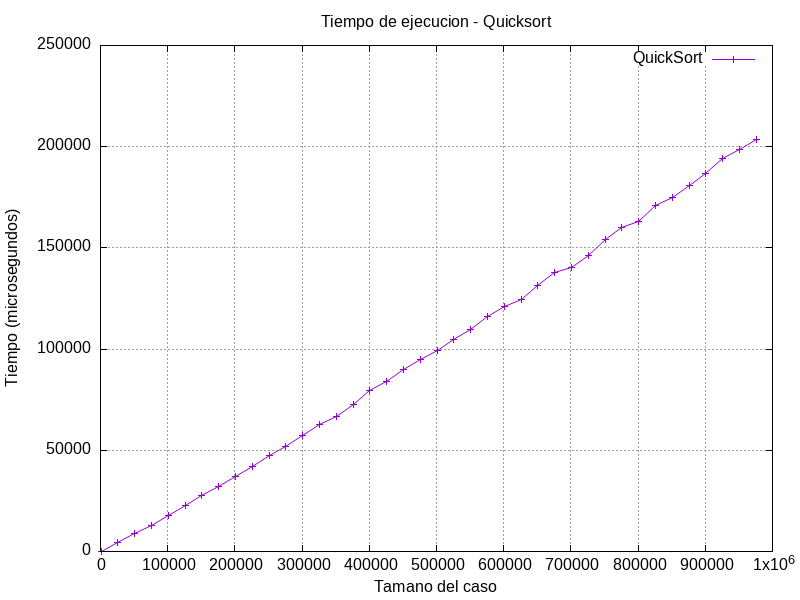
\includegraphics[width=\linewidth]{Graficas/Quicksort.png}
	\caption{Ajuste por regresión de \textit{QuickSort}.}
\end{figure}

\subsubsection{BubbleSort}
\paragraph{Eficencia teórica}
\paragraph{Eficiencia práctica}

A continuación mostramos las gráficas resultantes de ejecutar el algoritmo \textit{BubbleSort}
sobre tamaños empezando desde 1.000 hasta 10.000 con saltos de 1.000:

\begin{table}[H]
	\centering
	\resizebox{\textwidth}{!}{%
		\begin{tabular}{|c|c|c|c|}
			\hline
			\textbf{Tam.caso}                                  & \textbf{Tiempo (us)} & \textbf{$K=$ Tiempo/$f(n)$} & \textbf{Tiempo teórico estimado = $K\cdot f(n)$} \\
			\hline
			1000                                               & 2476                 & 0.002476                    & 1768.2078                                        \\
			2000                                               & 6132                 & 0.003066                    & 7020.8312                                        \\
			3000                                               & 14902                & 0.004967                    & 15913.8072                                       \\
			4000                                               & 25212                & 0.00157575                  & 28921.3271                                       \\
			5000                                               & 38002                & 0.0016004                   & 46326.8609                                       \\
			6000                                               & 50808                & 0.001468                    & 63655.4809                                       \\
			7000                                               & 70807                & 0.00173455                  & 86642.1199                                       \\
			8000                                               & 109808               & 0.0013735                   & 116315.2989                                      \\
			9000                                               & 148216               & 0.0016489                   & 143224.2831                                      \\
			10000                                              & 269088               & 0.00182917                  & 176820.7946                                      \\
			\hline
			\multicolumn{2}{l}{\textbf{Media aritmética de K}} & \textbf{0.001768}                                                                                     \\
			\hline
		\end{tabular}%
	}
	\caption{Resultados de tiempos y estimaciones de BubbleSort.}
	\label{tab:resultados}
\end{table}

\begin{figure}[H]
	\centering
	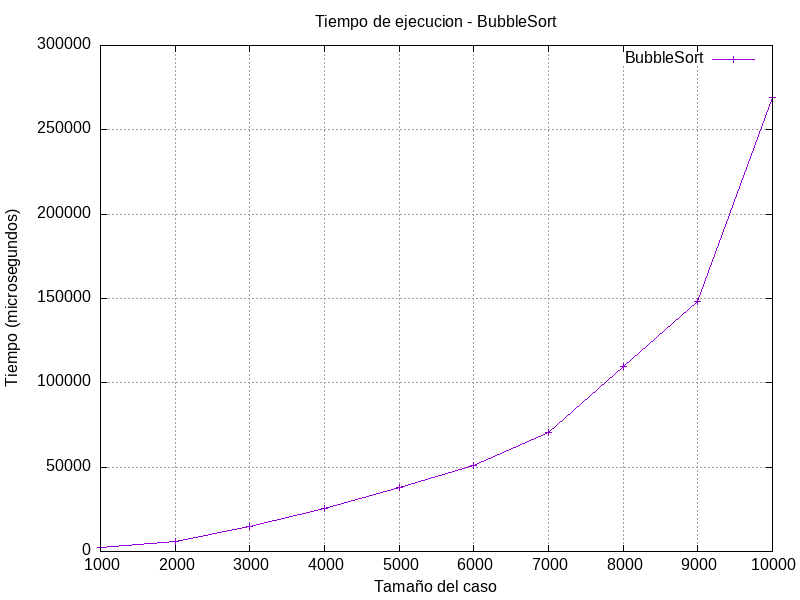
\includegraphics[width=\linewidth]{Graficas/Bubble.png}
	\caption{Ajuste por regresión de \textit{BubbleSort}.}
\end{figure}


\subsubsection{MergeSort}
\paragraph{Eficiencia teórica}
\paragraph{Eficiencia práctica}

A continuación mostramos las gráficas resultantes de ejecutar el algoritmo \textit{MergeSort}
sobre tamaños empezando desde 10.000 hasta 100.000 con saltos de 1.000:

\begin{table}[H]
	\centering
	\resizebox{\textwidth}{!}{%
		\begin{tabular}{|c|c|c|c|}
			\hline
			\textbf{Tam. Caso}                        & \textbf{Tiempo (us)} & \textbf{$K=$ Tiempo/$f(n)$} & \textbf{Tiempo teórico estimado = $K\cdot f(n)$} \\
			\hline
			10000                                     & 2220                 & 0.0555                      & 1054.6881                                        \\
			20000                                     & 1972                 & 0.0229247                   & 2268.1228                                        \\
			30000                                     & 3198                 & 0.0238099                   & 3541.4752                                        \\
			40000                                     & 4262                 & 0.0231527                   & 4853.7383                                        \\
			50000                                     & 5419                 & 0.0230646                   & 6194.9352                                        \\
			60000                                     & 6580                 & 0.0229517                   & 7559.1895                                        \\
			70000                                     & 7864                 & 0.0231869                   & 8942.6188                                        \\
			80000                                     & 9009                 & 0.0229677                   & 10342.4622                                       \\
			90000                                     & 10265                & 0.0230218                   & 11756.6574                                       \\
			100000                                    & 11546                & 0.023092                    & 13183.6024                                       \\
			\hline
			\multicolumn{2}{l}{\textbf{K promedio}} & \textbf{0.0263672}                                                                                \\
			\hline
		\end{tabular}%
	}
	\caption{Resultados de tiempos y estimaciones de MergeSort.}
	\label{tab:resultados}
\end{table}

\begin{figure}[H]
	\centering
	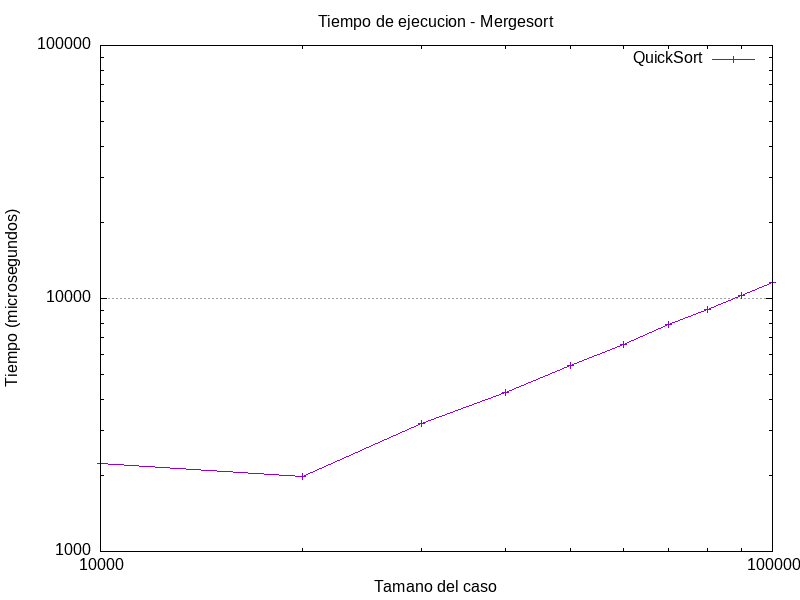
\includegraphics[width=\linewidth]{Graficas/Mergesort.png}
	\caption{Ajuste por regresión de \textit{MergeSort}.}
\end{figure}


\paragraph{Comparación}

A continuación se presenta la comparación del algoritmo QuickSort con BubbleSort:

\begin{figure}[H]
	\centering
	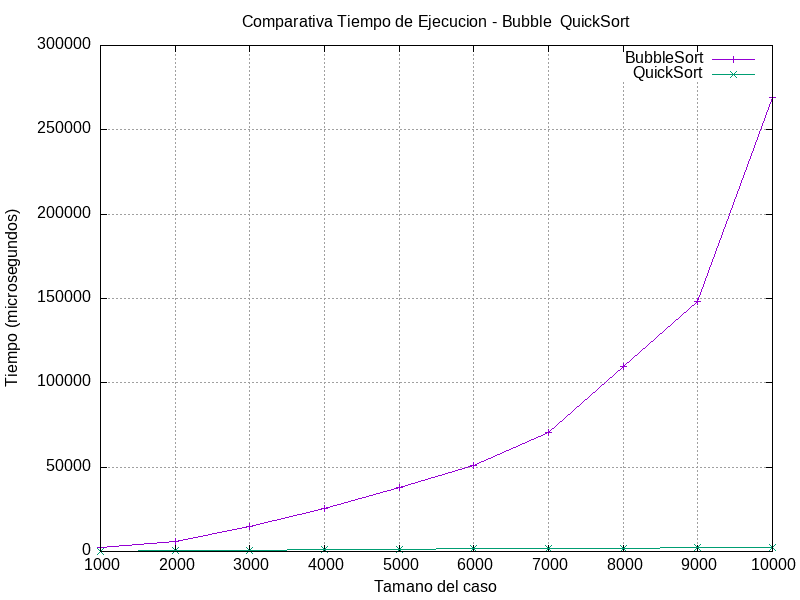
\includegraphics[width=\linewidth]{Graficas/ComparativaBubbleQuicksort.png}
	\caption{Comparación de QuickSort frente a BubbleSort.}
\end{figure}

Gracias al estudio de la eficiencia teórica ya aprendimos que el algoritmo QuickSort es más eficiente que
BubbleSort y ahora podemos ver esta mejora de eficiencia de manera gráfica, sin embargo observamos que para
casos de tamaños pequeños, la gŕafica de BubbleSort se encuentra por debajo que la de QuickSort, esto es debido
a que para dichos casos $O(n^2)$ está por debajo de $O(n\cdot \log (n))$.

Ahora veremos la comparación de QuickSort frente a MergeSort:

\begin{figure}[H]
	\centering
	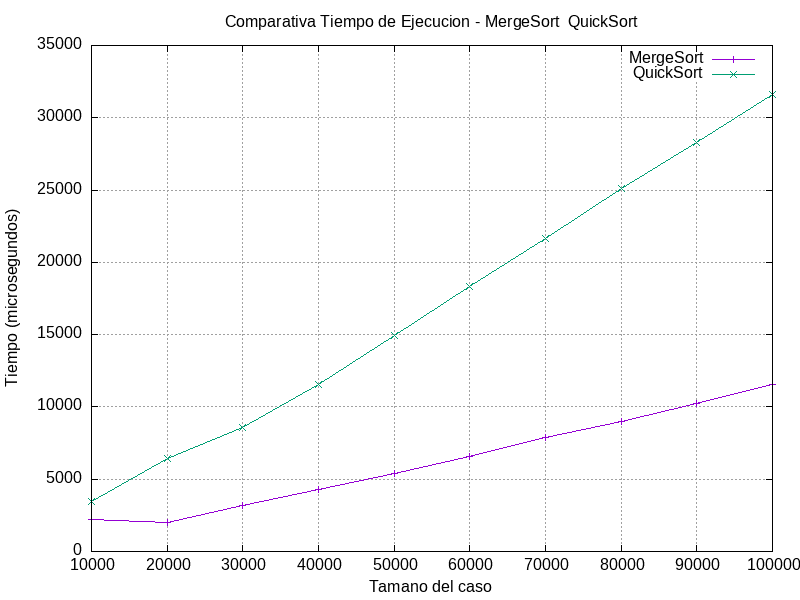
\includegraphics[width=\linewidth]{Graficas/ComparativaMergeyQuick.png}
	\caption{Comparación de QuickSort frente a MergeSort.}
\end{figure}


\subsection{Los números de Catalan}

\subsubsection{Versión recursiva}

\paragraph{Eficiencia práctica}

A continuación mostramos las gráficas resultantes de ejecutar el algoritmo \textit{Catalan Recursivo}
sobre tamaños empezando con 2 elementos hasta 21 con saltos de 1:

\begin{table}[H]
	\centering
	\resizebox{\textwidth}{!}{%
		\begin{tabular}{|c|c|c|c|}
			\hline
			\textbf{Tam.caso}                                  & \textbf{Tiempo (us)} & \textbf{K = Tiempo/f(n)} & \textbf{Tiempo teórico estimado = K \(\times\) f(n)} \\
			\hline
			2                                                  & 0                    & 0                        & 3.093061924                                          \\
			3                                                  & 0                    & 0                        & 6.186123848                                          \\
			4                                                  & 0                    & 0                        & 12.3722477                                           \\
			5                                                  & 0                    & 0                        & 24.74449539                                          \\
			6                                                  & 1                    & 0.015625                 & 49.48899078                                          \\
			7                                                  & 3                    & 0.0234375                & 98.97798157                                          \\
			8                                                  & 11                   & 0.04296875               & 197.9559631                                          \\
			9                                                  & 31                   & 0.060546875              & 395.9119263                                          \\
			10                                                 & 96                   & 0.09375                  & 791.8238525                                          \\
			11                                                 & 299                  & 0.145996094              & 1583.647705                                          \\
			12                                                 & 806                  & 0.196777344              & 3167.29541                                           \\
			13                                                 & 1904                 & 0.232421875              & 6334.59082                                           \\
			14                                                 & 5147                 & 0.314147949              & 12669.18164                                          \\
			15                                                 & 14977                & 0.457061768              & 25338.36328                                          \\
			16                                                 & 44252                & 0.675231934              & 50676.72656                                          \\
			17                                                 & 131750               & 1.005172729              & 101353.4531                                          \\
			18                                                 & 393200               & 1.499938965              & 202706.9063                                          \\
			19                                                 & 1181008              & 2.252593994              & 405413.8125                                          \\
			20                                                 & 3545546              & 3.381296158              & 810827.625                                           \\
			21                                                 & 10629085             & 5.068342686              & 1621655.25                                           \\
			\hline
			\multicolumn{2}{l}{\textbf{Media artimética de K}} & \textbf{0.773265481}                                                                                   \\
			\hline
		\end{tabular}
	}
	\caption{Resultados de tiempos y estimaciones de Catalan Recursivo.}
	\label{tab:tiempos}
\end{table}


\begin{figure}[H]
	\centering
	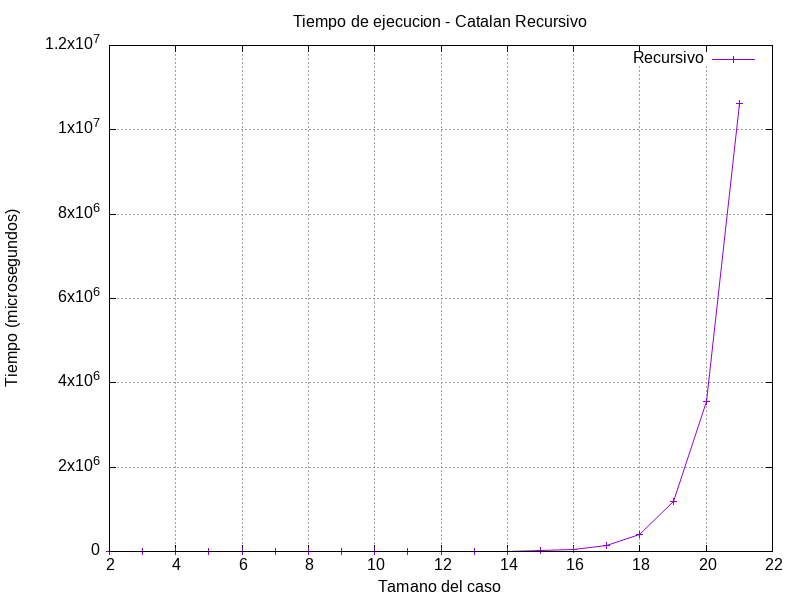
\includegraphics[width=\linewidth]{Graficas/CatalanRecursivo.png}
	\caption{Ajuste por regresión de \textit{Catalan Recursivo}.}
\end{figure}

\subsubsection{Versión iterativa (programación dinámica)}
\paragraph{Eficiencia práctica}

A continuación mostramos las gráficas resultantes de ejecutar el algoritmo \textit{Catalan Iterativo PD}
sobre tamaños empezando desde 20 hasta 10.000 con saltos de 350:

\begin{table}[H]
	\centering
	\resizebox{\textwidth}{!}{%
		\begin{tabular}{|c|c|c|c|}
			\hline
			\textbf{Tam.caso}                                  & \textbf{Tiempo (us)} & \textbf{K = Tiempo/f(n)} & \textbf{Tiempo teórico estimado = K \(\times\) f(n)} \\
			\hline
			20                                                 & 0                    & 0                        & 0.095902338                                          \\
			370                                                & 1                    & 0.002702703              & 1.774193253                                          \\
			720                                                & 3                    & 0.004166667              & 3.452484169                                          \\
			1070                                               & 5                    & 0.004672897              & 5.130775084                                          \\
			1420                                               & 9                    & 0.006338028              & 6.809065999                                          \\
			1770                                               & 9                    & 0.005084746              & 8.487356915                                          \\
			2120                                               & 11                   & 0.005188679              & 10.16564783                                          \\
			2470                                               & 12                   & 0.0048583                & 11.84393875                                          \\
			2820                                               & 14                   & 0.004964539              & 13.52222966                                          \\
			3170                                               & 16                   & 0.005047319              & 15.20052058                                          \\
			3520                                               & 17                   & 0.004829545              & 16.87881149                                          \\
			3870                                               & 20                   & 0.005167959              & 18.55710241                                          \\
			4220                                               & 22                   & 0.00521327               & 20.23539332                                          \\
			4570                                               & 23                   & 0.005032823              & 21.91368424                                          \\
			4920                                               & 26                   & 0.005284553              & 23.59197515                                          \\
			5270                                               & 27                   & 0.00512334               & 25.27026607                                          \\
			5620                                               & 29                   & 0.005160142              & 26.94855698                                          \\
			5970                                               & 31                   & 0.00519263               & 28.6268479                                           \\
			6320                                               & 33                   & 0.005221519              & 30.30513881                                          \\
			6670                                               & 34                   & 0.005097451              & 31.98342973                                          \\
			7020                                               & 36                   & 0.005128205              & 33.66172065                                          \\
			7370                                               & 39                   & 0.005291723              & 35.34001156                                          \\
			7720                                               & 40                   & 0.005181347              & 37.01830248                                          \\
			8070                                               & 42                   & 0.005204461              & 38.69659339                                          \\
			8420                                               & 44                   & 0.005225653              & 40.37488431                                          \\
			8770                                               & 45                   & 0.005131129              & 42.05317522                                          \\
			9120                                               & 47                   & 0.005153509              & 43.73146614                                          \\
			9470                                               & 39                   & 0.004118268              & 45.40975705                                          \\
			9820                                               & 42                   & 0.004276986              & 47.08804797                                          \\
			\hline
			\multicolumn{2}{l}{\textbf{Media artimética de K}} & \textbf{0.004795117}                                                                                   \\
			\hline
		\end{tabular}
	}
	\caption{Resultados de tiempos y estimaciones de Catalan iterativo PD.}
	\label{tab:tiempos}
\end{table}

\begin{figure}[H]
	\centering
	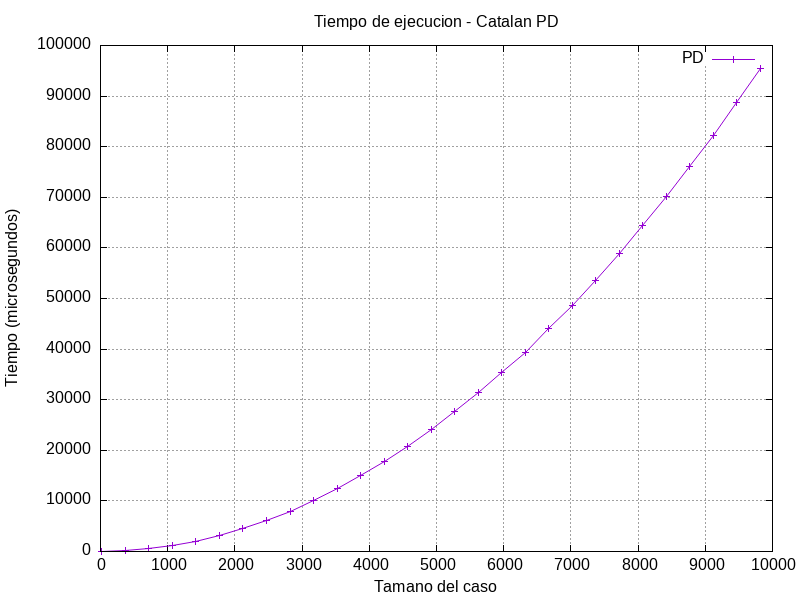
\includegraphics[width=\linewidth]{Graficas/CatalanPD_BIG_NUMBERS.png}
	\caption{Ajuste por regresión de \textit{Catalan Iterativo (programación dinámica)}.}
\end{figure}

\subsubsection{Versión iterativa directa usado el coeficiente binomial}
\paragraph{Eficiencia práctica}



A continuación mostramos las gráficas resultantes de ejecutar el algoritmo \textit{Catalan iterativo binomial}
sobre tamaños empezando con 20 hasta 10.000 con saltos de 350:

\begin{table}[H]
	\centering
	\resizebox{\textwidth}{!}{%
		\begin{tabular}{|c|c|c|c|}
			\hline
			\textbf{Tam.caso}                                  & \textbf{Tiempo (us)} & \textbf{K = Tiempo/f(n)} & \textbf{Tiempo teórico estimado = K \(\times\) f(n)} \\
			\hline
			20                                                 & 0                    & 0                        & 0.393360124                                          \\
			370                                                & 181                  & 0.001322133              & 134.6275026                                          \\
			720                                                & 651                  & 0.001255787              & 509.7947212                                          \\
			1070                                               & 1169                 & 0.00102105               & 1125.895016                                          \\
			1420                                               & 2052                 & 0.001017655              & 1982.928387                                          \\
			1770                                               & 3174                 & 0.001013119              & 3080.894834                                          \\
			2120                                               & 4551                 & 0.001012593              & 4419.794358                                          \\
			2470                                               & 6161                 & 0.001009851              & 5999.626957                                          \\
			2820                                               & 8003                 & 0.001006363              & 7820.392633                                          \\
			3170                                               & 10088                & 0.001003891              & 9882.091385                                          \\
			3520                                               & 12409                & 0.001001501              & 12184.72321                                          \\
			3870                                               & 15013                & 0.00100241               & 14728.28812                                          \\
			4220                                               & 17826                & 0.001000988              & 17512.7861                                           \\
			4570                                               & 20844                & 0.000998042              & 20538.21716                                          \\
			4920                                               & 24140                & 0.000997257              & 23804.58129                                          \\
			5270                                               & 27661                & 0.000995971              & 27311.8785                                           \\
			5620                                               & 31412                & 0.000994542              & 31060.10878                                          \\
			5970                                               & 35415                & 0.000993662              & 35049.27214                                          \\
			6320                                               & 39394                & 0.00098627               & 39279.36858                                          \\
			6670                                               & 43997                & 0.000988943              & 43750.3981                                           \\
			7020                                               & 48646                & 0.000987127              & 48462.36069                                          \\
			7370                                               & 53611                & 0.000987004              & 53415.25635                                          \\
			7720                                               & 58827                & 0.000987057              & 58609.0851                                           \\
			8070                                               & 64390                & 0.000988716              & 64043.84691                                          \\
			8420                                               & 70220                & 0.000990459              & 69719.54181                                          \\
			8770                                               & 76059                & 0.000988898              & 75636.16978                                          \\
			9120                                               & 82239                & 0.000988754              & 81793.73083                                          \\
			9470                                               & 88717                & 0.000989252              & 88192.22495                                          \\
			9820                                               & 95402                & 0.000989315              & 94831.65215                                          \\
			\hline
			\multicolumn{2}{l}{\textbf{Media artimética de K}} & \textbf{0.0009834}                                                                                     \\
			\hline
		\end{tabular}
	}
	\caption{Resultados de tiempos y estimaciones de Catalan Iterativo Binomial}
	\label{tab:tiempos}
\end{table}

\begin{figure}[H]
	\centering
	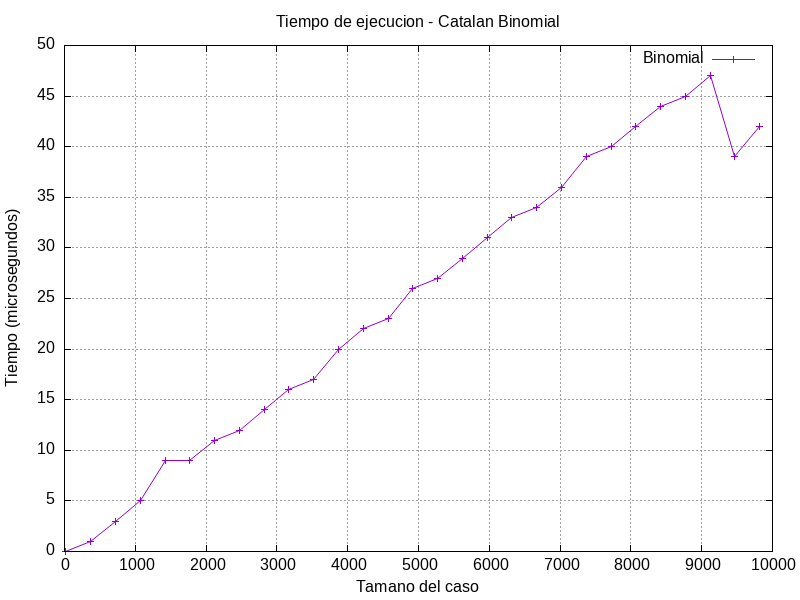
\includegraphics[width=\linewidth]{Graficas/CatalanBinomial_BIG_NUMBERS.png}
	\caption{Ajuste por regresión de \textit{Catalan Iterativo usando el Coeficiente Binomial}.}
\end{figure}

\paragraph{Comparación}

A continuación se presenta la comparación de los tres algoritmos de Catalan:

\begin{figure}[H]
	\centering
	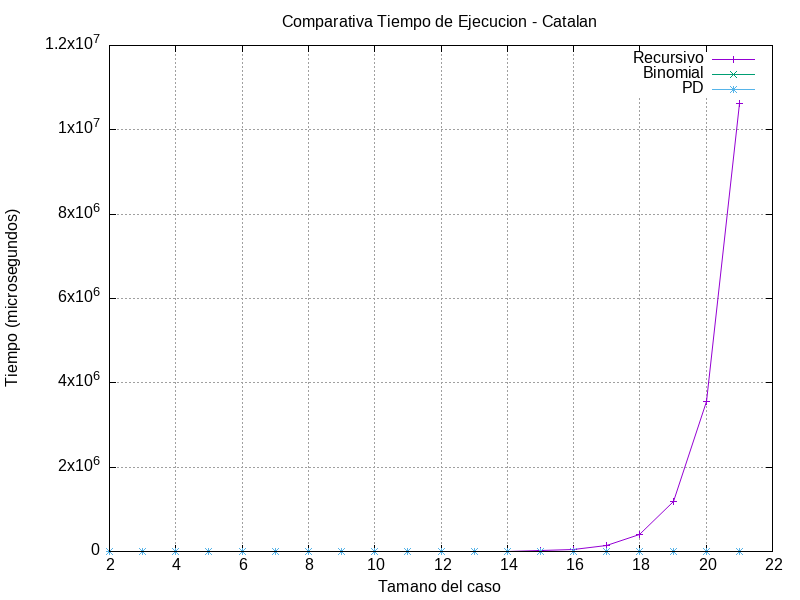
\includegraphics[width=\linewidth]{Graficas/ComparativaCatalan.png}
	\caption{Comparación de los algoritmos de Catalan.}
\end{figure}

También la comparativa en escala logarítmica:

\begin{figure}[H]
	\centering
	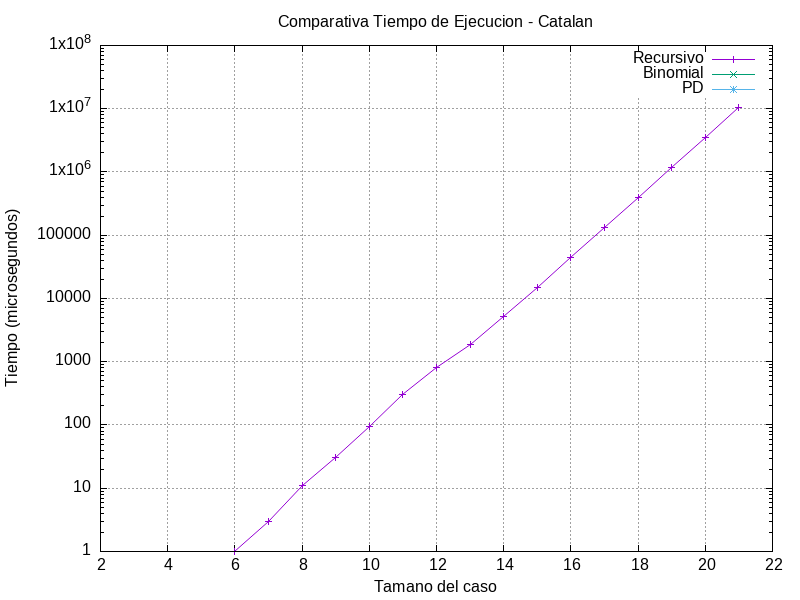
\includegraphics[width=\linewidth]{Graficas/ComparativaCatalan_LOGSCALE.png}
	\caption{Comparación de los algoritmos de Catalan en escala logarítmica.}
\end{figure}

\subsection{Las Torres de Hanoi}

\subsubsection{Versión recursiva}
\paragraph{Eficiencia teórica}

A continuación se presenta el código que hemos usado para hacer el análisis:

\begin{lstlisting}[language=C, caption={Código de Hanoi}]
void Hanoi(int n, char from_rod, char to_rod,
            char aux_rod)
{
    if (n == 0) {
        return;
    }
    Hanoi(n - 1, from_rod, aux_rod, to_rod);
    cout << "Move disk " << n << " from rod " << from_rod
         << " to rod " << to_rod << endl;
    Hanoi(n - 1, aux_rod, to_rod, from_rod);
}
\end{lstlisting}

Tras analizar el código hemos llegado a la siguiente fórmula de recurrencia:

\[
	H(n)=
	\begin{cases}
		0,             & \text{si } n = 0, \\[6pt]
		2\cdot H(n-1), & \text{si } n > 0
	\end{cases}
\]

Concluimos que en las dos llamadas recursivas de \textit{Hanoi}
se utiliza \textit{n - 1}, de donde sale $2\cdot H(n-1)$, y el caso base
0 ocurre cuando hay 0 discos.

Procedemos a resolver la ecuación:

\begin{align*}
	x - 2 = 0 \\
	x = 2
\end{align*}

Por tanto la solución es $(x -2)$, con multiplicidad 1, y expresando la
ecuación con coeficientes llegamos finalmente a:

\begin{equation*}
	c_{1}\cdot 2^{n}
\end{equation*}

De donde se deduce que Hanoi tiene una eficiencia de \textit{O}$(2^{n})$

\paragraph{Eficiencia práctica}

A continuación mostramos las gráficas resultantes de ejecutar el algoritmo \textit{Hanoi Recursivo}
sobre tamaños empezando con 5 elementos hasta 27 con saltos de 1:


\begin{table}[H]
	\centering
	\resizebox{\textwidth}{!}{%
		\begin{tabular}{|c|c|c|c|}
			\hline
			\textbf{Tam.caso}                                  & \textbf{Tiempo (us)} & \textbf{$K=$ Tiempo/$f(n)$} & \textbf{Tiempo teórico estimado = $K\cdot f(n)$} \\
			\hline
			5                                                  & 0                    & 0                           & 0.093463214                                      \\
			6                                                  & 0                    & 0                           & 0.186926427                                      \\
			7                                                  & 0                    & 0                           & 0.373852854                                      \\
			8                                                  & 0                    & 0                           & 0.747705708                                      \\
			9                                                  & 1                    & 0.001953125                 & 1.495411417                                      \\
			10                                                 & 3                    & 0.002929688                 & 2.990822834                                      \\
			11                                                 & 7                    & 0.003417969                 & 5.981645667                                      \\
			12                                                 & 15                   & 0.003662109                 & 11.96329133                                      \\
			13                                                 & 32                   & 0.00390625                  & 23.92658267                                      \\
			14                                                 & 61                   & 0.003723145                 & 47.85316534                                      \\
			15                                                 & 123                  & 0.003753662                 & 95.70633067                                      \\
			16                                                 & 244                  & 0.003723145                 & 191.4126613                                      \\
			17                                                 & 485                  & 0.003700256                 & 382.8253227                                      \\
			18                                                 & 974                  & 0.003715515                 & 765.6506454                                      \\
			19                                                 & 1937                 & 0.003694534                 & 1531.301291                                      \\
			20                                                 & 3867                 & 0.003687859                 & 3062.602582                                      \\
			21                                                 & 7632                 & 0.003639221                 & 6125.205163                                      \\
			22                                                 & 15199                & 0.003623724                 & 12250.41033                                      \\
			23                                                 & 30871                & 0.00368011                  & 24500.82065                                      \\
			24                                                 & 60305                & 0.003594458                 & 49001.6413                                       \\
			25                                                 & 120463               & 0.003590077                 & 98003.28261                                      \\
			26                                                 & 240884               & 0.003589451                 & 196006.5652                                      \\
			27                                                 & 482162               & 0.003592387                 & 392013.1304                                      \\
			\hline
			\multicolumn{2}{l}{\textbf{Media aritmética de K}} & \textbf{0.002920725}                                                                                  \\
			\hline
		\end{tabular}%
	}
	\caption{Resultados de tiempos y estimaciones de Hanoi Recursivo.}
	\label{tab:resultados}
\end{table}

La gráfica resultante es:
\begin{figure}[H]
	\centering
	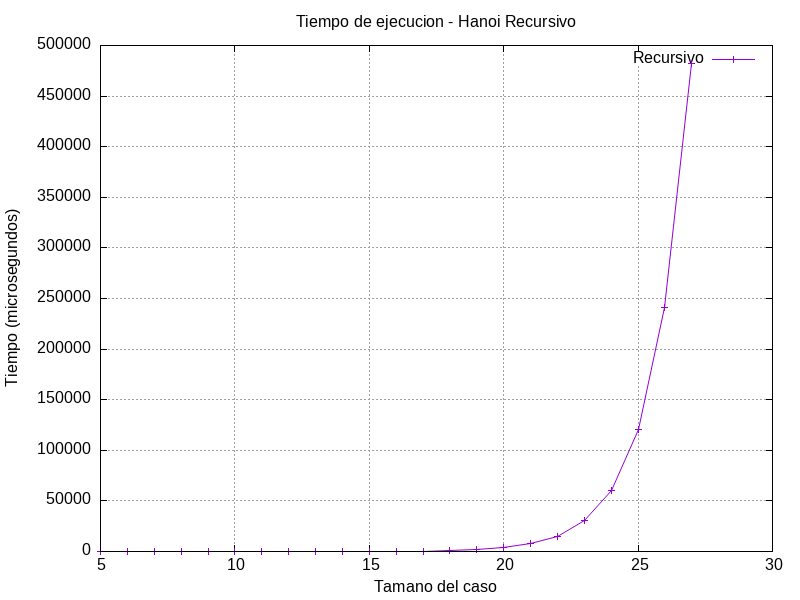
\includegraphics[width=\linewidth]{Graficas/HanoiRecursivo.png}
	\caption{Ajuste por regresión de \textit{Hanoi Recursivo}.}
\end{figure}


\subsubsection{Versión iterativa usando una pila}

\paragraph{Eficiencia teórica}

A continuación se presenta el código que hemos usado para hacer el análisis:

\begin{lstlisting}[language=C, caption={Código de Hanoi Iterativo con pila}]
	void moveDisk(int a, int b)
	{
		if (!stacks[a].empty() && (stacks[b].empty() || stacks[a].top() < stacks[b].top()))
		{
			stacks[b].push(stacks[a].top());
			stacks[a].pop();
		}
	}
	 
	void Hanoi(int n)
	{
	 
		int src = 0, aux = 1, dest = 2;
		for (int i = n; i > 0; i--)
			stacks[src].push(i);
	 
		int totalMoves = (1 << n) - 1;
		if (n % 2 == 0)
			swap(aux, dest);
	 
		for (int i = 1; i <= totalMoves; i++)
		{
			if (i % 3 == 0)
				moveDisk(aux, dest);
			else if (i % 3 == 1)
				moveDisk(src, dest);
			else
				moveDisk(src, aux);
		}
	}
\end{lstlisting}

Tras analizar el código vemos que:

El primer bucle claramente tiene una eficiencia de \textit{O}(n) ya que vemos que comienza con $i=n$ (el número de discos)
y va decrementando hasta llegar a 0.\\

El segundo bucle recorre desde $i=1$ hasta llegar a la variable totalMoves que se obtiene con la función
$(1 \ll n) - 1$ que equivale a $2^n - 1$ por tanto el segundo bucle tiene una eficiencia de \textit{O}($2^n$).\\

Por tanto, por la regla del máximo, al no estar los bucles anidados obtenemos que la eficiencia total de la función es \textit{O}($2^n$).\\

\paragraph{Eficiencia práctica}

A continuación mostramos las gráficas resultantes de ejecutar el algoritmo \textit{Hanoi Con Pila}
sobre tamaños empezando con 5 elementos hasta 27 con saltos de 1:

\begin{table}[H]
	\centering
	\resizebox{\textwidth}{!}{%
		\begin{tabular}{|c|c|c|c|}
			\hline
			\textbf{Tam.caso}                                  & \textbf{Tiempo (us)} & \textbf{K = Tiempo/f(n)} & \textbf{Tiempo teórico estimado = K \(\times\) f(n)} \\
			\hline
			5                                                  & 1                    & 0.03125                  & 0.967404925                                          \\
			6                                                  & 2                    & 0.03125                  & 1.934809851                                          \\
			7                                                  & 3                    & 0.0234375                & 3.869619701                                          \\
			8                                                  & 7                    & 0.02734375               & 7.739239402                                          \\
			9                                                  & 16                   & 0.03125                  & 15.4784788                                           \\
			10                                                 & 30                   & 0.029296875              & 30.95695761                                          \\
			11                                                 & 63                   & 0.030761719              & 61.91391522                                          \\
			12                                                 & 124                  & 0.030273438              & 123.8278304                                          \\
			13                                                 & 249                  & 0.030395508              & 247.6556609                                          \\
			14                                                 & 499                  & 0.030456543              & 495.3113218                                          \\
			15                                                 & 999                  & 0.030487061              & 990.6226435                                          \\
			16                                                 & 2044                 & 0.031188965              & 1981.245287                                          \\
			17                                                 & 4107                 & 0.031333923              & 3962.490574                                          \\
			18                                                 & 8119                 & 0.030971527              & 7924.981148                                          \\
			19                                                 & 16236                & 0.030967712              & 15849.9623                                           \\
			20                                                 & 32090                & 0.030603409              & 31699.92459                                          \\
			21                                                 & 64218                & 0.030621529              & 63399.84918                                          \\
			22                                                 & 127909               & 0.030495882              & 126799.6984                                          \\
			23                                                 & 256123               & 0.030532241              & 253599.3967                                          \\
			24                                                 & 513154               & 0.030586362              & 507198.7935                                          \\
			25                                                 & 1026528              & 0.030592918              & 1014397.587                                          \\
			26                                                 & 2059635              & 0.030690953              & 2028795.174                                          \\
			27                                                 & 4098268              & 0.030534476              & 4057590.348                                          \\
			\hline
			\multicolumn{2}{l}{\textbf{Media aritmética de K}} & \textbf{0.030231404}                                                                                   \\
			\hline
		\end{tabular}
	}
	\caption{Resultados de tiempos y estimaciones teóricas del Hanoi Iterativo con Pila.}
	\label{tab:tiempos}
\end{table}

La gráfica resultante es:
\begin{figure}[H]
	\centering
	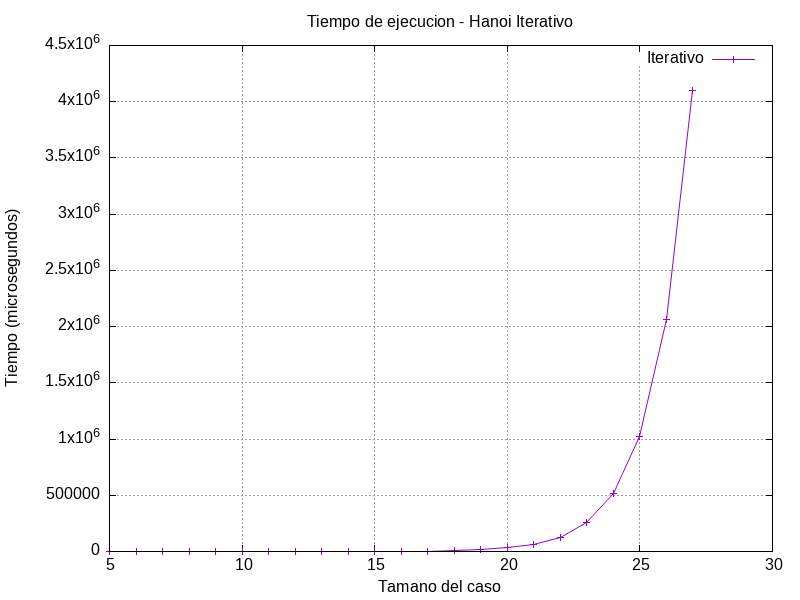
\includegraphics[width=\linewidth]{Graficas/HanoiIterativo.png}
	\caption{Ajuste por regresión de \textit{Hanoi Iterativo}.}
\end{figure}


\subsubsection{Versión iterativa sin usar la pila}

\paragraph{Eficiencia teórica}

A continuación se presenta el código que hemos usado para hacer el análisis:

\begin{lstlisting}[language=C, caption={Código de Hanoi Iterativo sin pila}]
	void moveDisksBetweenTwoPoles(struct Stack *src, struct Stack *dest, char s, char d) {
		int pole1TopDisk = pop(src);
		int pole2TopDisk = pop(dest);
	
		if (pole1TopDisk == INT_MIN) {
			push(src, pole2TopDisk);
		} else if (pole2TopDisk == INT_MIN) {
			push(dest, pole1TopDisk);
		} else if (pole1TopDisk > pole2TopDisk) {
			push(src, pole1TopDisk);
			push(src, pole2TopDisk);
		} else {
			push(dest, pole2TopDisk);
			push(dest, pole1TopDisk);
		}
	}
	
	void tohIterative(int num_of_disks, struct Stack *src, struct Stack *aux, struct Stack *dest) {
		char s = 'S', d = 'D', a = 'A';
		if (num_of_disks % 2 == 0) swap(d, a);
	
		int total_num_of_moves = pow(2, num_of_disks) - 1;
		for (int i = num_of_disks; i >= 1; i--) push(src, i);
	
		for (int i = 1; i <= total_num_of_moves; i++) {
			if (i % 3 == 1) moveDisksBetweenTwoPoles(src, dest, s, d);
			else if (i % 3 == 2) moveDisksBetweenTwoPoles(src, aux, s, a);
			else moveDisksBetweenTwoPoles(aux, dest, a, d);
		}
	}
\end{lstlisting}

Tras analizar el código vemos que:

El primer bucle claramente tiene una eficiencia de \textit{O}(n) ya que vemos que comienza con $i=n$ (el número de discos)
y va decrementando hasta llegar a 1.\\

El segundo bucle recorre desde $i=1$ hasta llegar a la variable total\_num\_of\_moves que se obtiene con la función
pow(2, num\_of\_disks) - 1 que equivale a $2^n - 1$ por tanto el segundo bucle tiene una eficiencia de \textit{O}($2^n$).\\

Por tanto, por la regla del máximo, al no estar los bucles anidados obtenemos que la eficiencia total de la función es \textit{O}($2^n$).\\

\paragraph{Eficiencia práctica}

A continuación mostramos las gráficas resultantes de ejecutar el algoritmo \textit{Hanoi Iterativo sin pila}
sobre tamaños empezando con 5 elementos hasta 27 con saltos de 1:

\begin{table}[H]
	\centering
	\resizebox{\textwidth}{!}{%
		\begin{tabular}{|c|c|c|c|}
			\hline
			\textbf{Tam.caso}                                  & \textbf{Tiempo (us)} & \textbf{K = Tiempo/f(n)} & \textbf{Tiempo teórico estimado = K \(\times\) f(n)} \\
			\hline
			5                                                  & 12                   & 0.375                    & 0.952186895                                          \\
			6                                                  & 1                    & 0.015625                 & 1.904373791                                          \\
			7                                                  & 1                    & 0.0078125                & 3.808747582                                          \\
			8                                                  & 3                    & 0.01171875               & 7.617495164                                          \\
			9                                                  & 7                    & 0.013671875              & 15.23499033                                          \\
			10                                                 & 14                   & 0.013671875              & 30.46998065                                          \\
			11                                                 & 29                   & 0.014160156              & 60.93996131                                          \\
			12                                                 & 65                   & 0.015869141              & 121.8799226                                          \\
			13                                                 & 132                  & 0.016113281              & 243.7598452                                          \\
			14                                                 & 257                  & 0.015686035              & 487.5196905                                          \\
			15                                                 & 496                  & 0.015136719              & 975.0393809                                          \\
			16                                                 & 924                  & 0.014099121              & 1950.078762                                          \\
			17                                                 & 1906                 & 0.014541626              & 3900.157524                                          \\
			18                                                 & 3906                 & 0.014900208              & 7800.315048                                          \\
			19                                                 & 7271                 & 0.013868332              & 15600.63010                                          \\
			20                                                 & 14782                & 0.014097214              & 31201.26019                                          \\
			21                                                 & 29515                & 0.014073849              & 62402.52038                                          \\
			22                                                 & 58605                & 0.013972521              & 124805.0408                                          \\
			23                                                 & 118189               & 0.014089227              & 249610.0815                                          \\
			24                                                 & 236037               & 0.014068902              & 499220.1630                                          \\
			25                                                 & 471250               & 0.014044344              & 998440.3261                                          \\
			26                                                 & 944599               & 0.014075622              & 1996880.652                                          \\
			27                                                 & 1890864              & 0.014088035              & 3993761.304                                          \\
			\hline
			\multicolumn{2}{l}{\textbf{Media aritmética de K}} & \textbf{0.02975584}                                                                                    \\
			\hline
		\end{tabular}
	}
	\caption{Resultados de tiempos y estimaciones teóricas de Hanoi Iterativo con Pila.}
	\label{tab:tiempos}
\end{table}
La gráfica resultante es:
\begin{figure}[H]
	\centering
	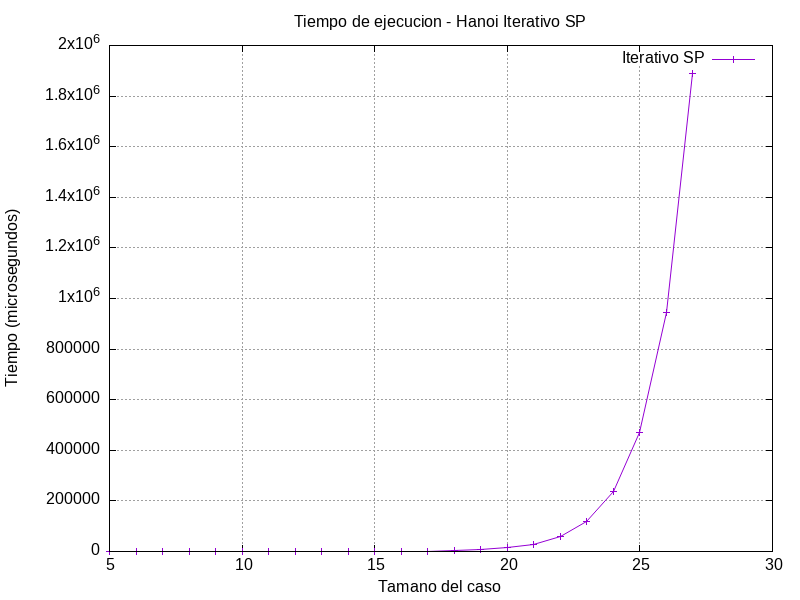
\includegraphics[width=\linewidth]{Graficas/HanoiIterativoSP.png}
	\caption{Ajuste por regresión de \textit{Hanoi Iterativo Sin Pila}.}
\end{figure}

\paragraph{Comparación}

A continuación se presenta la comparación de los tres algoritmos de Hanoi:

\begin{figure}[H]
	\centering
	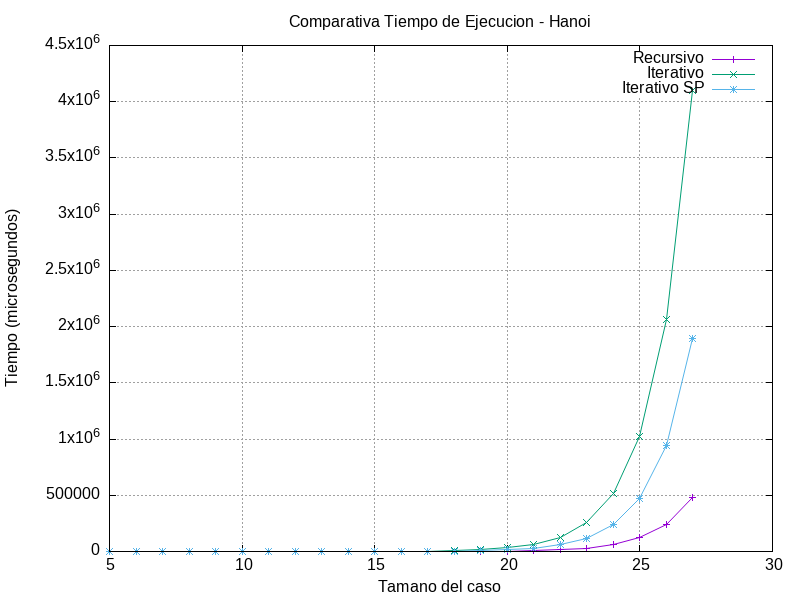
\includegraphics[width=\linewidth]{Graficas/ComparativaHanoi.png}
	\caption{Comparación de los algoritmos de Hanoi.}
\end{figure}

También la comparativa en escala logarítmica:

\begin{figure}[H]
	\centering
	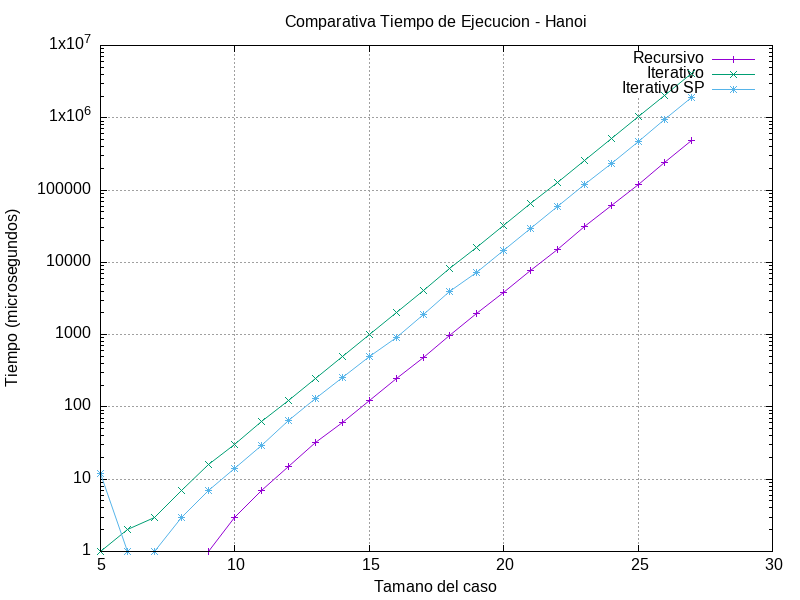
\includegraphics[width=\linewidth]{Graficas/ComparativaHanoi_LOGSCALE.png}
	\caption{Comparación de los algoritmos de Hanoi en escala logarítmica.}
\end{figure}

\section{Conclusión}
En conclusión, somos sudorosos.




\end{document}